\chapter{Data Analysis}

\MyQuote{In physics, you don't have to go around making trouble for yourself - nature
does it for you.}{Frank Wilczek}

QCD jets are the most common hard objects observed at hadron colliders, with
their cross section exceeding any other physics process by orders of magnitude.
Measurement of inclusive jet cross section thus provide the first test for both
QCD predictions and the detector performance. LHC Run II should open new
kinematic region with expectation of observation of jets with $\pt$ in $\TeV$
region.

This chapter describes the details of the inclusive jet double cross section
analysis.

\section{Data Characteristics}

Data used in this thesis are Monte Carlo generated events of $pp$ collisions at
the center-of-mass energy $\sqrt{s} = 13\TeV$ by \textsc{Pythia8}
(?citace?) event generator using CT10 PDFs (?citace?) and ATLAS underlying event
tune AU2 (?citace?). QCD calculations are done only to the leading order in
\textsc{Pythia8}. The response of the ATLAS detector on these events was
calculated with ?\textsc{Geant4}? (?citace?) software toolkit.

Particles were recombined using anti-$k_t$ jet algorithm with parameter $R=0.4$.
There are parton jets reconstructed from the \textsc{Pythia8} output, which
further in this thesis are denoted truth jets, and next to them, there are the
signal jets reconstructed from the output of \textsc{Geant4} detector
simulation from the topological cell clusters. 

Signal jets were calibrated using \textsc{ApplyJetCalibration} (?citace?)
library version 3.28 and configuration parameters were loaded from the
\texttt{JES\_Full2012dataset\_May2014.config} with calibration sequence
\texttt{JetArea\_Residual\_EtaJES}. In next signal jets denotes the signal
calibrated jets.

Generated events are divided into JZXW samples according to
the leading truth jet $\pt$. These samples differ in event weight which is for
the whole event calculated as the product of cross section, filter efficiency,
inverse number of events and additional weight factor which is for each event
stored in \texttt{EventInfoAux} container. Concrete values for datasets used in
this theses are given in Table \ref{tab:JZXW}.  

\begin{table}
  \centering
  \begin{tabular}{|c|rcr|c|c|c|}
    \hline 
     JZXW & \multicolumn{3}{|c|}{$\pt$ range (GeV)} & Cross-section (fb) & Filter Efficiency & \# envents  \\ 
    \hline
    \hline
		 JZ0W &     0 & - &    20 & 7.8420e+13 & 9.7193e-01 & 3498000 \\ 
    \hline
		 JZ1W &    20 & - &    80 & 7.8420e+13 & 2.7903e-04 & 2998000 \\
    \hline
		 JZ2W &    80 & - &   200 & 5.7312e+10 & 5.2261e-03 & 500000  \\
    \hline
		 JZ3W &   200 & - &   500 & 1.4478e+09 & 1.8068e-03 & 499500  \\
    \hline
		 JZ4W &   500 & - &  1000 & 2.3093e+07 & 1.3276e-03 & 477000  \\
    \hline
		 JZ5W &  1000 & - &  1500 & 2.3793e+05 & 5.0449e-03 & 499000  \\
    \hline
		 JZ6W &  1500 & - &  2000 & 5.4279e+03 & 1.3886e-02 & 493500  \\
    \hline
		 JZ7W &  2000 & + &       & 9.4172e+02 & 6.7141e-02 & 497000  \\
    \hline 
  \end{tabular}
  \caption{The cross-sections, filter efficiency and number of events for the JZXW samples which differ in the leading truth jet $\pt$.}
  \label{tab:JZXW}
\end{table}

Analysis uses jets with transverse momentum $\pt > 15\GeV$ and rapidity $|y| <
4$ and is done in double binning in $\pt$ and $|y|$ with the following edges

\small
\begin{align}
  \pt = \, &15:20:25:35:45:55:70:85:100:116:134:152:172:194:216:240:264:290: \nonumber \\
        &318:346:376:408:442:478:516:556:598:642:688:736:786:838:894:952: \nonumber \\
        &1012:1076:1162:1310:1530:1992:2300:2800:3400:4100:5000:6000:7200 \GeV \nonumber \\
  |y| = \, &0.0:0.5:1.0:1.5:2.0:2.5:3.0:3.5:4.0
  \label{eq:Binning}
\end{align}
\normalsize

\section{Event Selection}

In this section the jet selection criteria and matching of truth with signal
jets are described. The former is needed to cut those jets (or those events)
off, which were misinterpreted by the detector, by the later the inputs for the
unfolding procedure are obtained. Description of the unfolding procedure will
follow in the next section. More details including graphical display and
numerical results for procedures described in this section are given in Appendix
\ref{App:CutAndMatchingResults}.

\subsection{Jet Cuts}
\label{SubSec:JetCuts}

\begin{itemize}
  \item \textbf{$\mathbf{\pt}$ Cut}

    By this cut those signal and truth jets with $\pt < 15 \GeV$ were removed from
    the list.

  \item \textbf{$\mathbf{y}$ Cut}
    
    By this cut those signal and truth jets with $|y| > 4$ were removed from the
    list.

  \item \textbf{Zero jet (0jet) Cut}

    If there was no signal or truth jet left in the event after previous cuts,
    the whole event was skipped.
    
  \item \textbf{Leading Ration (LR) Cut}

    In this cut the signal and truth jets with the highest $\pt$ were used. If
    there were only one signal jet left, the ratio $LR = \pt^{signal,leading} /
    \pt^{truth,leading}$ was calculated. If there were two signal jets, instead
    of $\pt^{signal,leading}$ the average $\pt$ of two leading signal jets was
    calculated. If $LR > 1$, $LR$ was replaced by its inverse value. If $LR <
    0.6$ the whole event was skipped.

\end{itemize}

Numbers of signal and truth jets removed in each step are shown in Table
\ref{tab:CutAndMatchingEfficiency}, where also the cut efficiencies for individual
JZXW samples are shown. The impact of each cut on jet $\pt$ spectrum of signal
and truth jets is displayed in Figure \ref{fig:Cutting}. 

It can be seen that the most important cut is the 0jet cut which removes
approximately $80\,\%$ of signal jets in JZ0W sample whereas the truth jets
remain intact. According to Table \ref{tab:JZXW} for event from the JZ0W sample
the leading truth jet $\pt < 20 \GeV$ which has no longer to hold for signal
jets which were in some cases reconstructed with $\pt \sim 100 \GeV$. Because of
Monte Carlo event weight of events from JZ0W sample is dominant over event
weights of other JZXW samples by several orders, the misreconstructed signal
jets from JZ0W sample were parasitizing on the observed $\pt$ spectrum of signal
jets as can be seen from top of the Figure \ref{fig:Cutting}.

\subsection{Jet Matching}
\label{SubSec:JetMatching}

To find, how the truth jets are reconstructed by the detector, the jet matching
has to be done, i.e. for each truth jet it is needed to find signal jet whom
could the original truth jet become. 

For each pair $(i,j)$ of signal and truth jet, the quantity $dR_{ij} =
\sqrt{d\phi_{ij}^2 + dy_{ij}^2}$ was calculated with $d\phi_{ij} =
\phi_i^{signal} - \phi_j^{truth}$ and $dy_{ij} = y_i^{signal} - y_j^{truth}$.
The minimum was found between all of $dR_{ij}$'s. If this minimum led under the
defined cutoff $\min(dR_{ij}) = dR_{pq} < dR^{cutoff} = 0.2$, the jets $(p,q)$
were matched and further not assumed in matching procedure. This continued until
condition $\min(dR_{ij}) < dR^{cutoff}$ was not satisfied or all of the signal
or truth jets were matched.

Numbers of signal and truth jets, both matched and unmatched are shown in Table
\ref{tab:CutAndMatchingEfficiency} where also the matching efficiencies for
individual JZXW samples are shown. In Figure \ref{fig:Matching} there are
compared $\pt$ spectra of matched and unmatched signal and truth jets with $\pt$
spectra of all signal and truth jets respectively, whereas in Figure
\ref{fig:MatchedUnmatched} the comparison between $\pt$ spectra of signal and
truth jets are shown for matched and unmatched jets separately.

It can be seen that for JZ(1-7)W samples, there is much more unmatched signal
jets, than is the unmatched truth jets. Looking back at the statistics of the
$\pt$ cut, the reason is, that more than a half of truth jets has $\pt < 15
\GeV$ in every JZXW sample, which does not hold for the signal jets. There is
much more signal jets in statistics than is the truth jets. 

From the top of the figure \ref{fig:MatchedUnmatched} showing the contribution
of matched jets to $\pt$ spectra, it can be seen, that starting with
$\pt>25\GeV$, $\pt$ spectra of signal jets overwhelms those of truth jets.
Taking into account the fact, that $\pt$ spectra of matched signal and matched
truth jets are obtained from the same number of jets, this can seem to be a
little bit confusing. The reason is, that some signal jets overflow the $\pt$
range defined by the JZXW sample and that each event is filled with weight
defined by the JZXW sample, which with increasing $\pt$ falls down.

\section{Unfolding}

Summarizing the results of the previous section, all events saved in Monte Carlo
simulated data firstly underwent the series of four cutoffs to obtain the set of
jets denoted signal and truth jets. Both signal and truth jets were split into
two categories depending on successful matching - there is correspondence $1:1$
between matched signal and matched truth jets. Signal jets, which were not
matched, formed the unmatched signal jets, and similarly set of unmatched truth
jets was created. All these 6 sets of jets are needed by the unfolding procedure
which description follows in this section.

\begin{figure}[h]
  \centering
  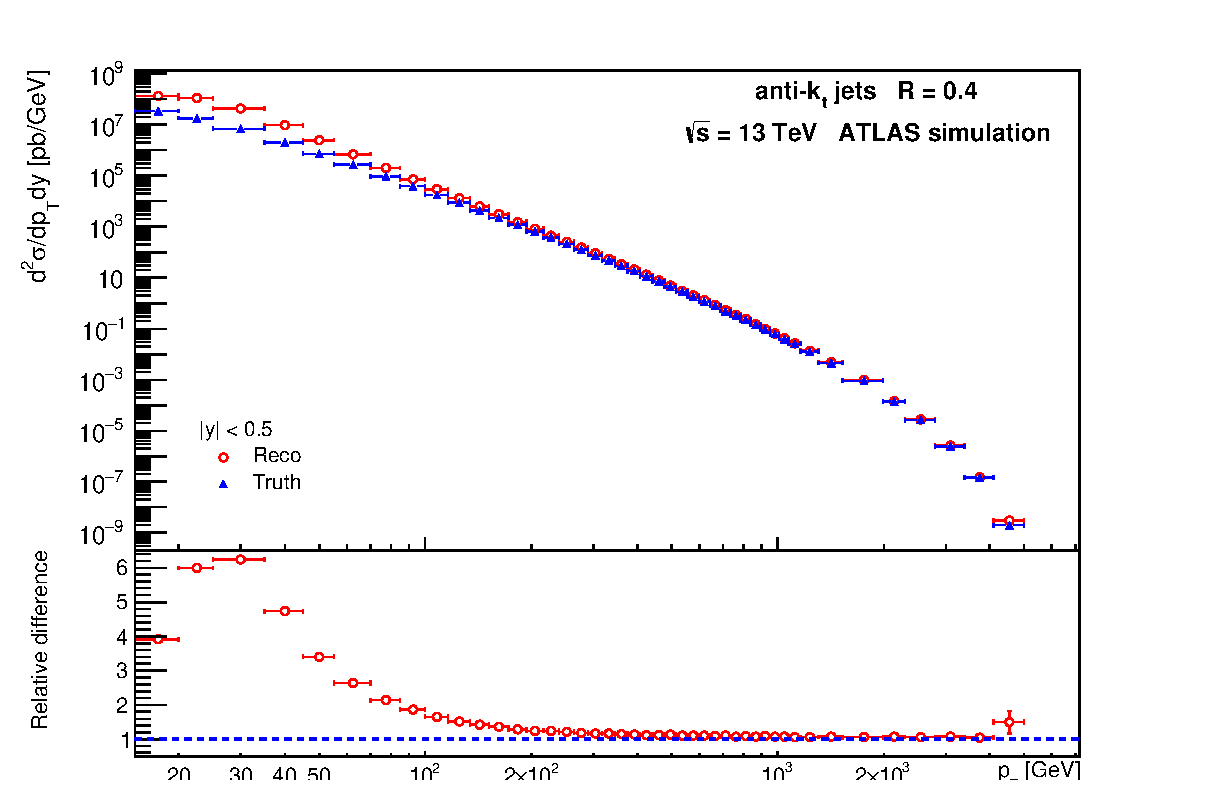
\includegraphics[width=\textwidth]{{Chapter3/SignalVSTruth}.eps}
  \caption{Comparison of $\pt$ spectra of signal and truth jets, which survived
  four steps of cutoff. Each bin was divided by its width so $y$-axis has
  physical meaning of differential cross section in $\pt$.
  Bottom graph contains the relative difference between signal and truth
  differential cross section in $\pt$.} 
  \label{fig:SignalVSTruth}
\end{figure}

Figure \ref{fig:SignalVSTruth} shows the $\pt$ spectra of signal and truth jets.
It can be seen, that observed $\pt$ spectrum, represented by the signal jets,
differs from the $\pt$ spectrum theoretically expected which is represented by
the $\pt$ spectrum of truth jets. Unfolding should transform the observed $\pt$
spectrum to the spectrum theoretically expected. If this transformation would be
done on real data, it should preserve additional structures, which are presented
in data, but not included by the theory.

The main ingredient for the unfolding procedure is the transfer matrix $A_{ij}$
which cells are proportional to number of signal jets in bin $i$ with a matched
truth jet that was generated in bin $j$. Example of unfolding matrix is shown in
Figure \ref{fig:UnfoldingMatrixDetail} where only matched signal and truth jets
both with rapidity $|y|<0.5$ were used. 

\begin{figure}[h]
  \centering
  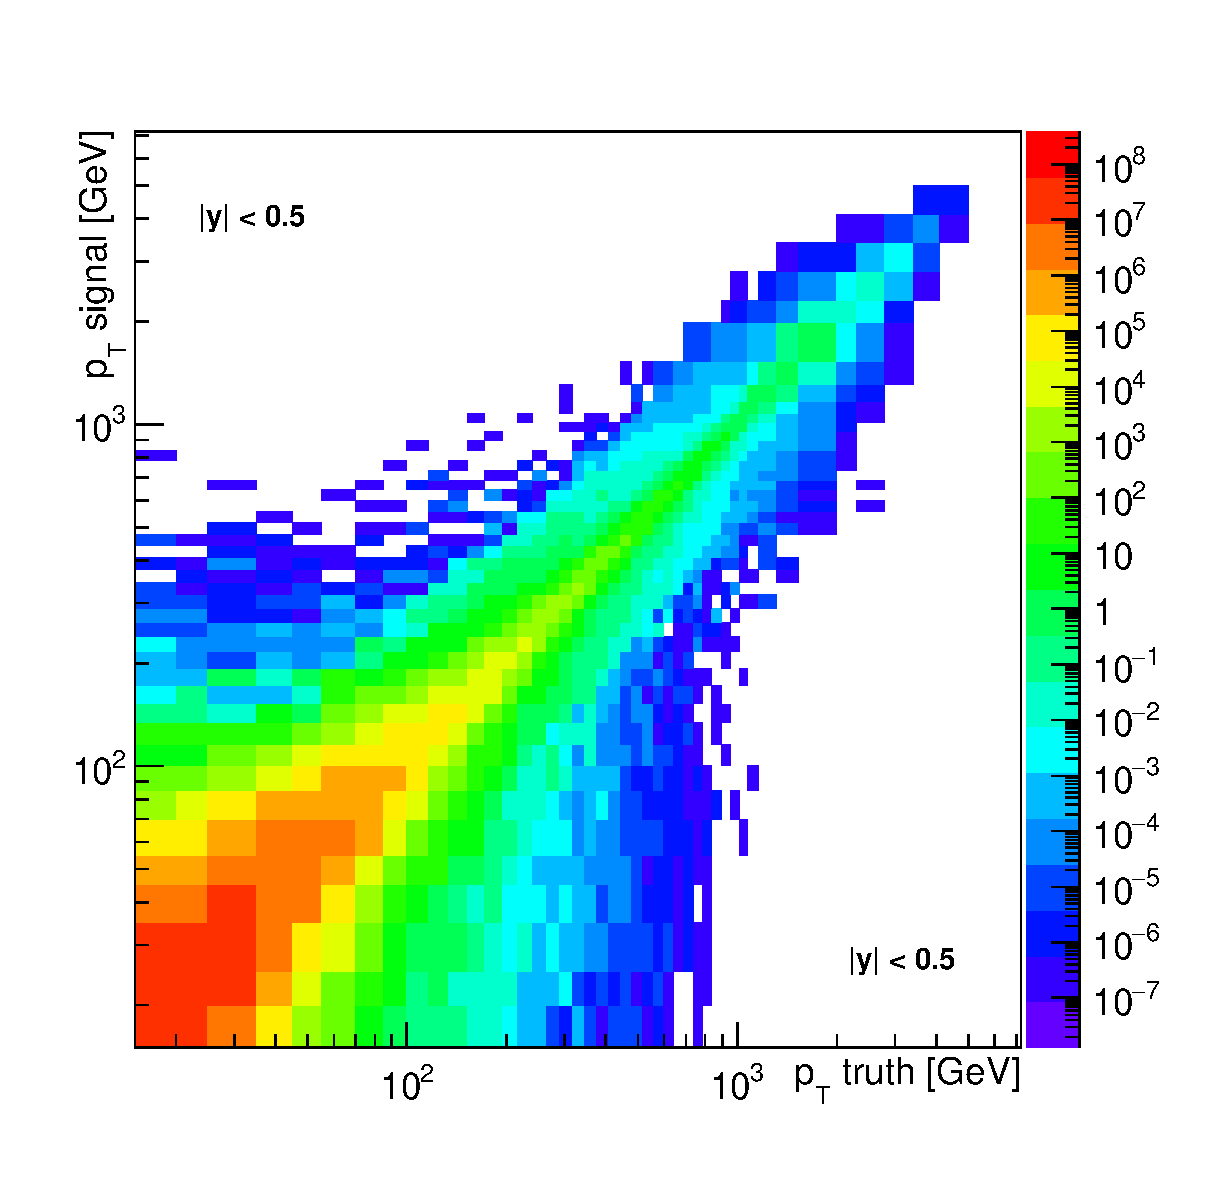
\includegraphics[width=\textwidth]{{Chapter3/Unfold_matrix_firstBin}.eps}
  \caption{Unfolding matrix for matched signal and truth jets with rapidity
  $|y|<0.5$. Each cell is proportional to the number of jets with truth $\pt$
  in range determined by the $x$-axis which were reconstructed to the signal jets
  with $\pt$ determined by the $y$-axis. White space signalize no input.}
  \label{fig:UnfoldingMatrixDetail}
\end{figure}

In this thesis the double binning \ref{eq:Binning} is used which complicates
the situation because the matched signal jet can simply migrate of the
transfer matrix from Figure \ref{fig:UnfoldingMatrixDetail}, when its rapidity
$|y|>0.5$ and when it was matched with truth jet with $|y|<0.5$. To these cases
could be treat, the transfer matrix was redefined in a way which can be easily seen
from Figure \ref{fig:UnfoldingMatrixAll} where the marked square represents the
previous unfolding matrix from Figure \ref{fig:UnfoldingMatrixDetail}.

\begin{figure}[h]
  \centering
  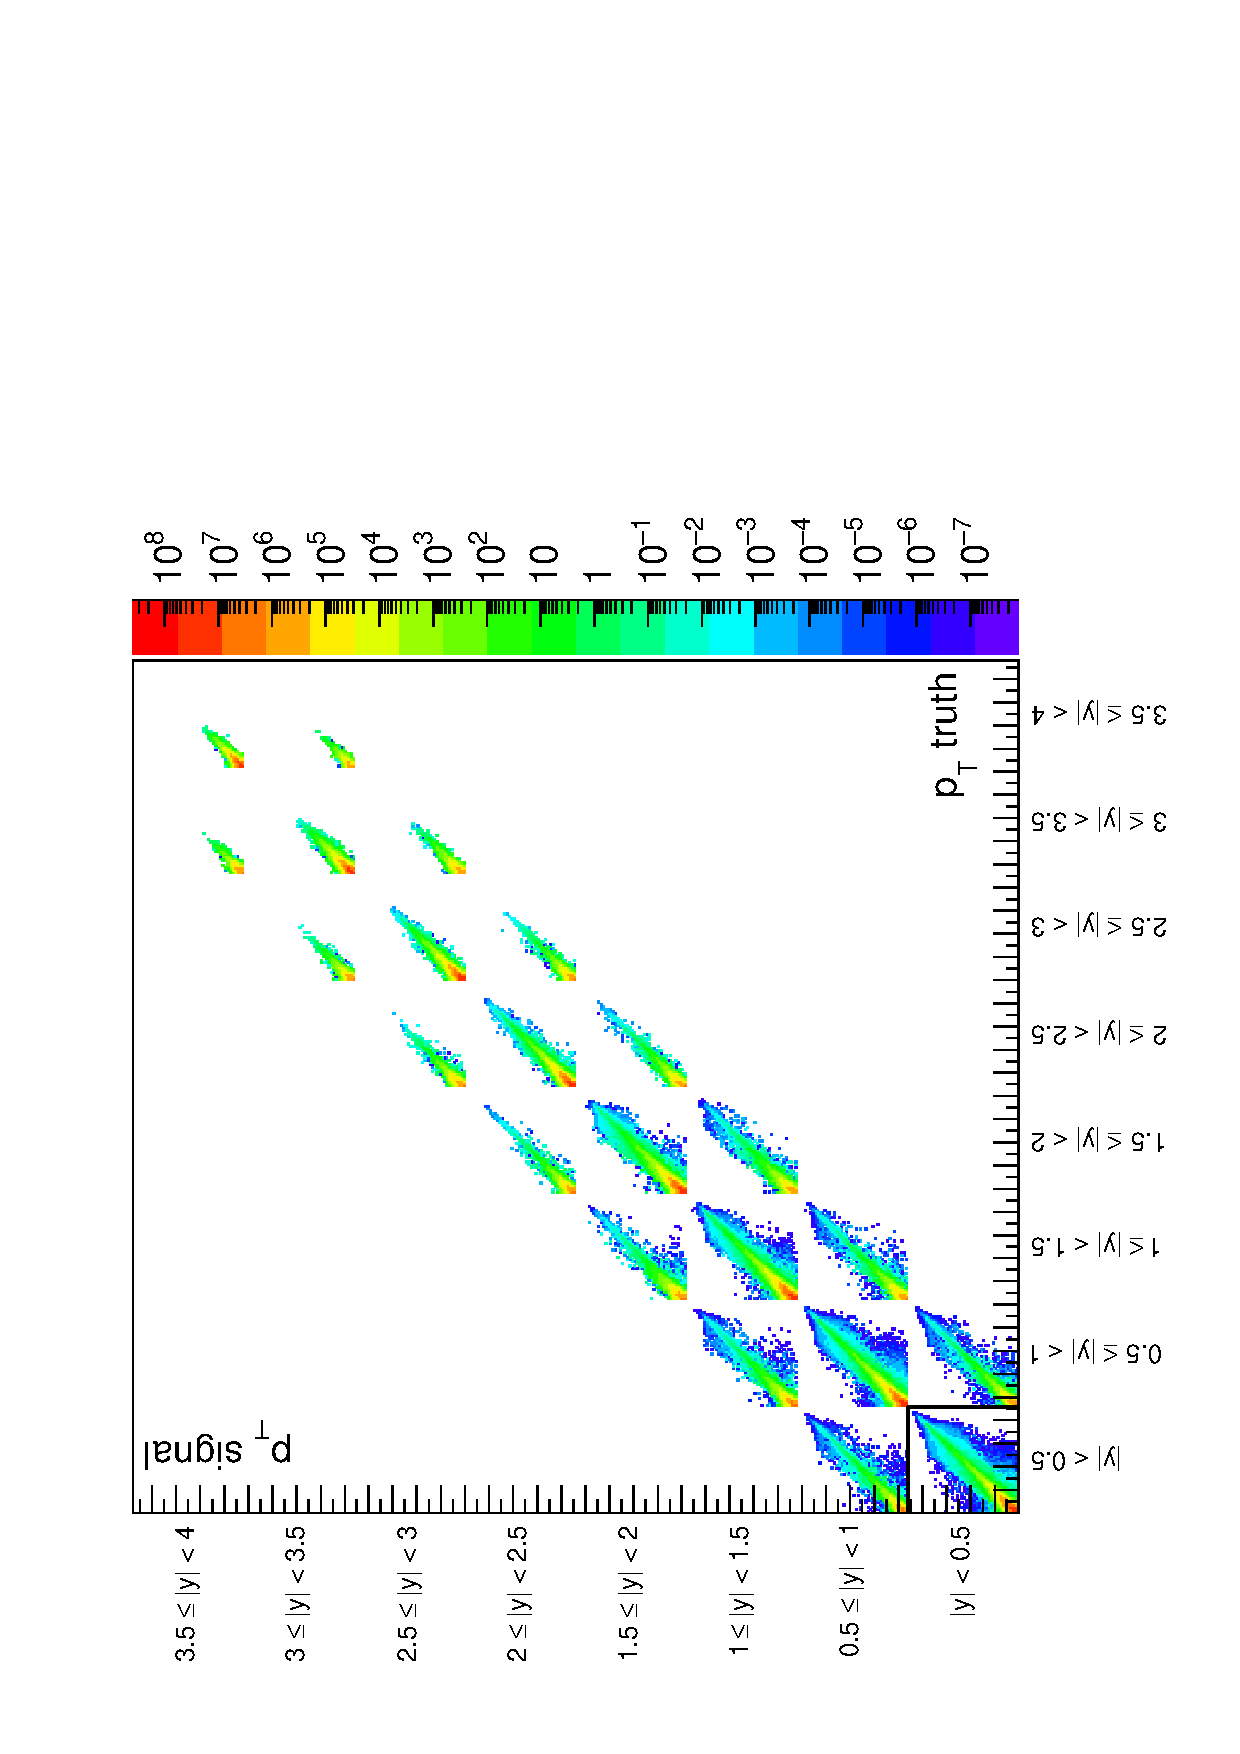
\includegraphics[width=\textwidth]{{Chapter3/Unfold_matrix_all}.eps}
  \caption{Unfolding matrix for all matched signal and truth jets. Each cell is
  proportional to the number of jets with truth $\pt$ and rapidity $y$
  determined by the $x$-axis, which were reconstructed to the signal jets with
  $\pt$ and $y$ determined by the $y$-axis. Marked square in $|y|<0.5$ region is
  shown in Figure \ref{fig:UnfoldingMatrixDetail}. Projection of this matrix on
  the $x$ and $y$-axis corresponds to the $\pt$ spectrum of truth and signal jets
  for corresponding rapidity bin respectively.}
  \label{fig:UnfoldingMatrixAll}
\end{figure}

The main diagonal of the unfolding matrix contains the dominant elements
corresponding to the correct reconstruction of the truth jet and meaning that
there is no significant bias in $\pt$ of matched signal and matched truth jets.
Next to the main diagonal, there are two minor diagonals representing the
migration of matched jets between different rapidity bins. All of these three
diagonals are smeared thanks to the final detector resolution in $\pt$. 

Next to the transfer matrix, numbers of matched and unmatched signal and truth
jets are needed for each $(y,\pt)$ bin by unfolding procedure. These serve for
calculation of matching efficiency which is the key ingredient for final
reweighting of reconstructed $\pt$ spectrum. The Iterative Dynamical Stabilized
(IDS) (?citace?) unfolding method was used in this thesis and the unfolding
procedure was iterated once.

Comparison of unfolded $\pt$ spectrum for $|y|<0.5$ rapidity bin is compared
with $\pt$ spectra of signal and truth jets in Figure \ref{fig:Unfolding0},
results for other rapidity bins are shown in Appendix
\ref{App:UnfoldingResults}. It can be seen, that the unfolded spectrum match the
truth spectrum up to the systematic error less than $5\,\%$.

\begin{figure}[h]
  \centering
  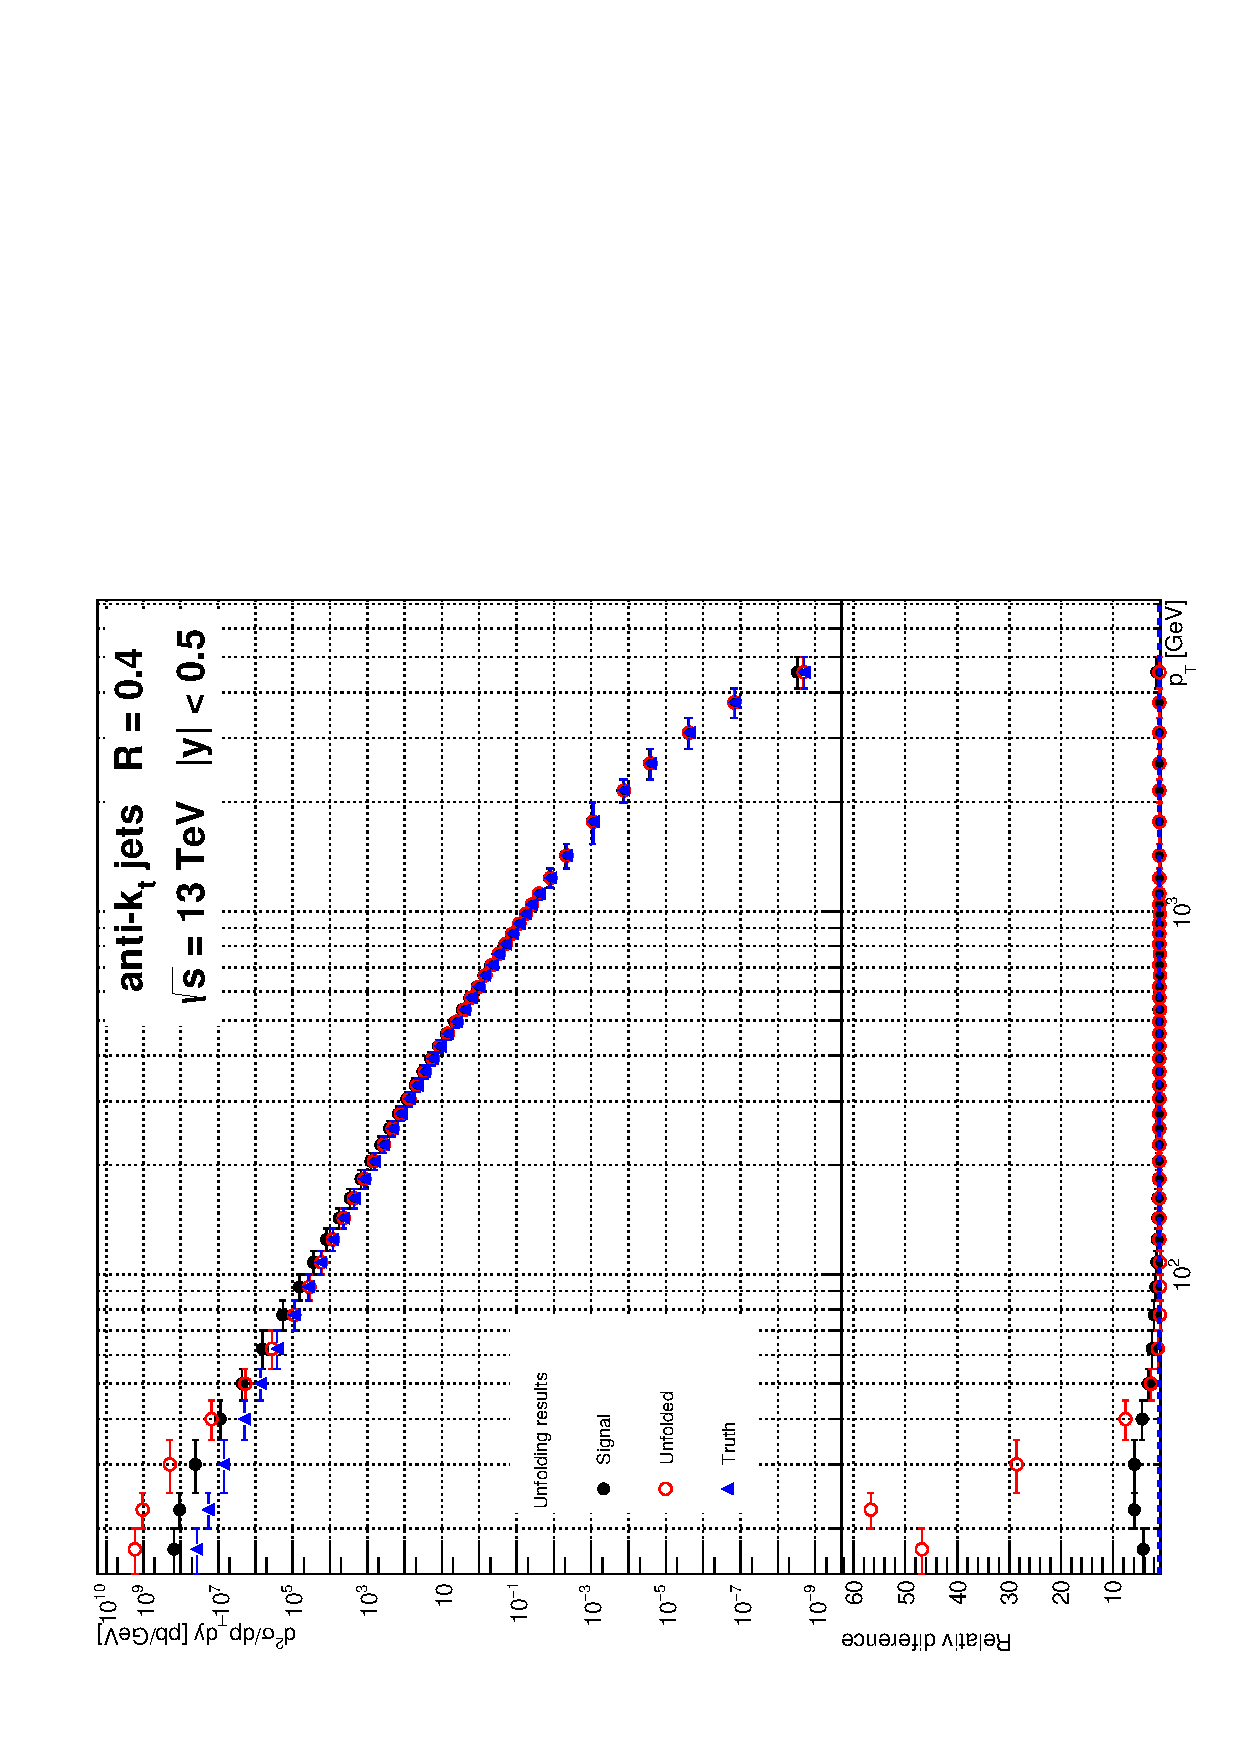
\includegraphics[width=\textwidth]{{Chapter3/Signal_VS_Unfold_VS_Truth_abs(y)0-0.5}.eps}
  \caption{Comparison of spectra of signal jets and unfolded spectra of signal
  jets with the spectrum of truth jets for $|y|<0.5$ rapidity bin. Each bin was
  divided by its width so the $y$-axis has meaning of double differential cross
  section in $\pt$ and $y$. The graph at bottom shows the relative difference
  between signal or unfolded spectrum and the truth spectrum.}
  \label{fig:Unfolding0}
\end{figure}


\section{Comparison with Prediction}

Unfolded $\pt$ spectrum obtained by the way described in previous section, was
compared with $\pt$ spectrum obtained by the NLO QCD calculations ?(?citace?)?
using ?PDF?. The result is for rapidity bin $|y|<0.5$ shown at Figure
\ref{fig:CompareUnfoldPred0}, results for other rapidity bins are shown in 
Appendix \ref{App:UnfoldingAndPrediction}. 

\begin{figure}[h]
  \centering
  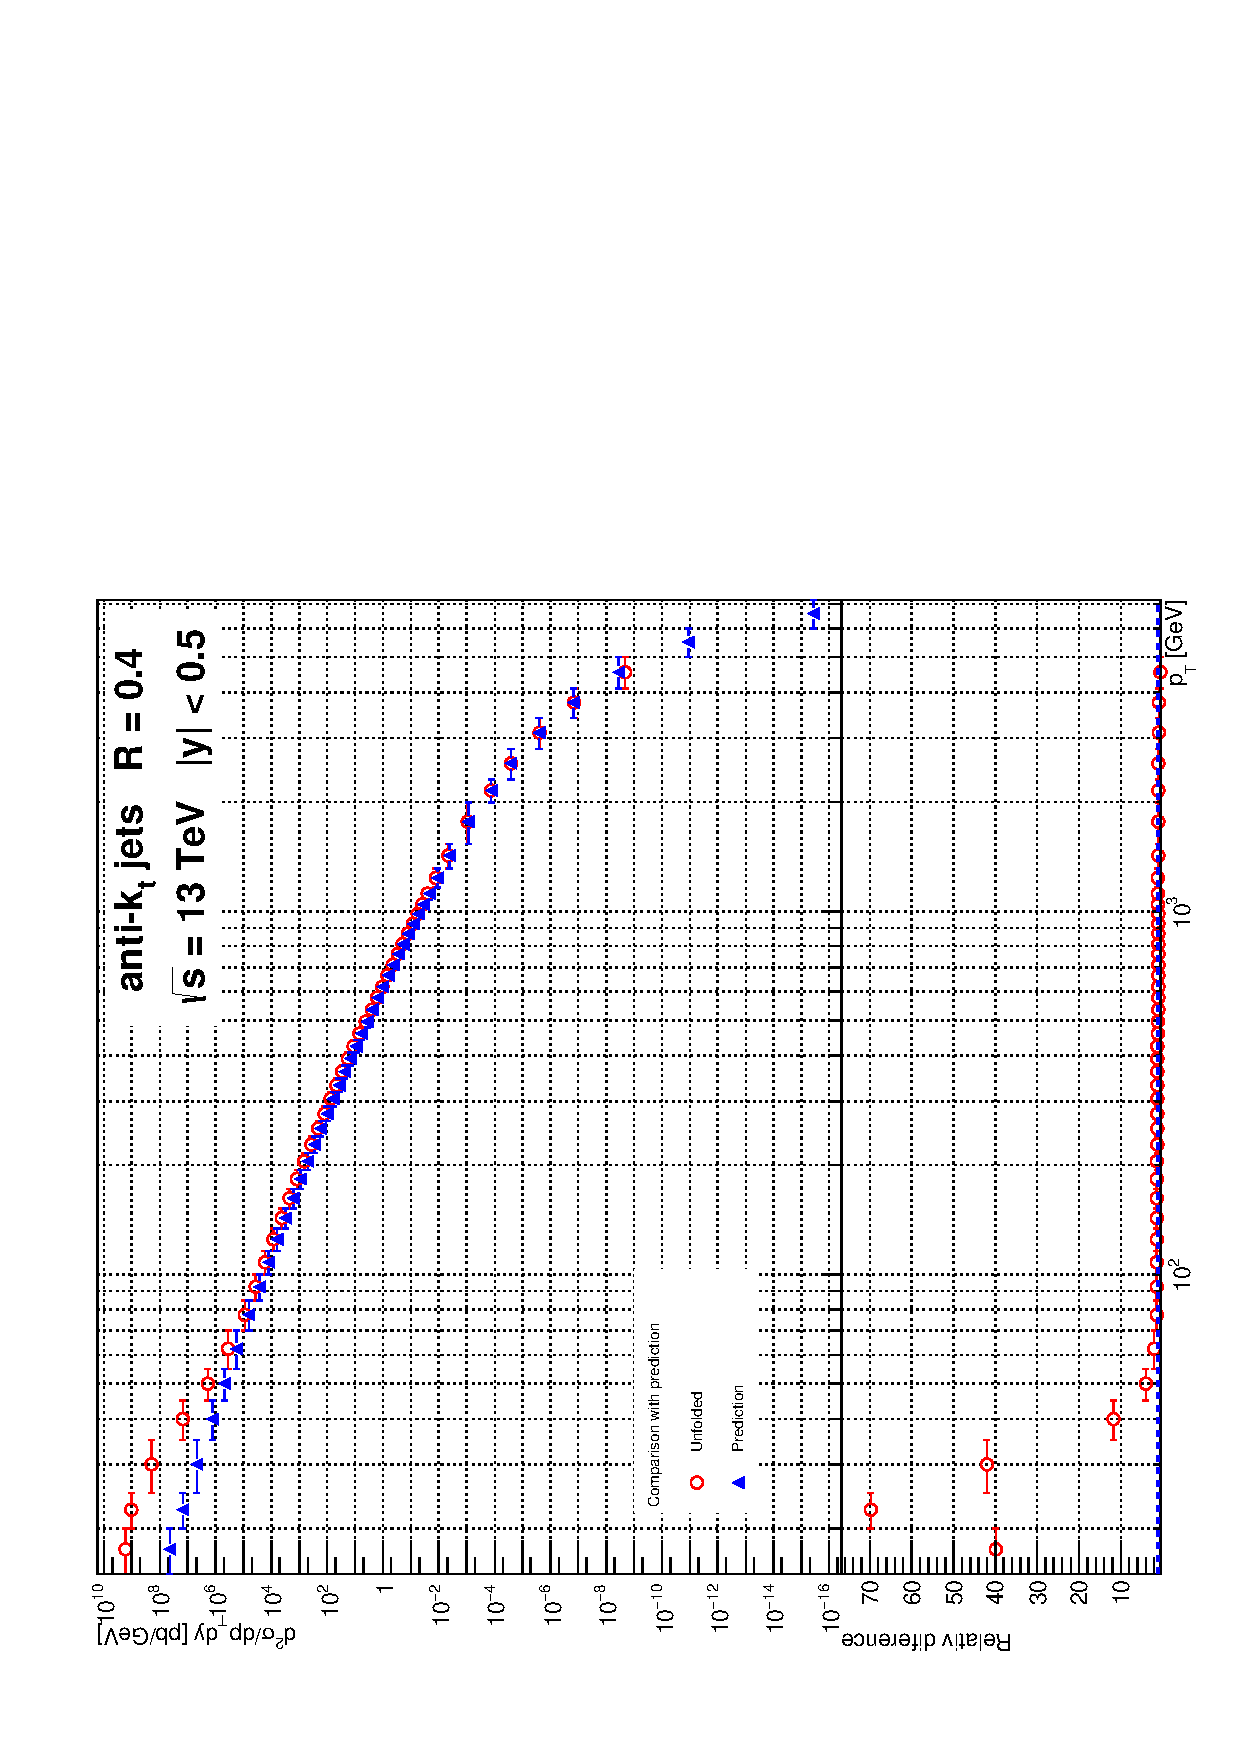
\includegraphics[width=\textwidth]{{Chapter3/Unfolded_VS_Prediciton_abs(y)0-0.5}.eps}
  \caption{Unfolded double differential cross section of inclusive jets in
  $\pt$ and rapidity $y$ compared to the NLO QCD prediction for $|y|<0.5$
  rapidity bin. At the bottom the relative difference between unfolded and
  predicted cross section is shown. }
  \label{fig:CompareUnfoldPred0}
\end{figure}

From the figures it follows, that there will be more jets observed with $\pt <
500\GeV$ than it is theoretically expected. This is because the reduced bunch
crossing time and increased luminosity will lead to increase of both underlying
events and pileup. This will increase the electronic noise in detector cells,
which will be misinterpreted by the detector either as increased jet energy or
as completely new unphysical jet. 

This effect becomes negligible as jet $\pt$ increases. For jets with rapidity
$|y|<2$ and $\pt > 500\GeV$ there is deviation $<10\,\%$ between the $\pt$
spectra obtained by the Monte Carlo simulations and the theoretical prediction.
For higher rapidity region $|y|>2$ there is significant drop-off in Monte Carlo
prediction against the theoretical prediction about more than $>10\,\%$.
